\chapter{Fundamentals}
\label{sec:fundamentals}

For a better understanding of error detection in HPE fundamentals are discussed in this section. 

\section{Human pose estimation}

There is a wide variety of how humans can interact with computers. Ranging from early punch cards to touch screens, the methods have evolved to be more natural and intuitive. In recent years, the use of cameras has become more popular, since they require no physical contact with a computer and therefore allow users to seamlessly interact with an application.

\paragraph{Pose visualisation}

Different methods to estimate the pose of a human have been developed, such as OpenPose, or Nuitrack. Depending on the usage of the pose estimation, different methods are used to visualise the pose of a human. These visualisations may provide different information about the pose of a human.

There are mainly three different ways the human pose can be visualised. The first and most basic way is to visualise the pose as a kinematic representation, in which a "skeleton" with bones and joints is used to represent the pose of a human. The skeleton is made up of joints, which are connected by bones. The number of joints and bones can vary, for example, the representation shown in figure \ref{fig:pose_representation}(a) uses 15 joints and 14 bones. The representation of a joint in the data varies, but it is usually a 2D point on the image plane or 3D point in space for example in a point cloud. In some cases, the joint representation is provided with a keypoint orientation that enables the clear representation of all degrees of freedoms joints have\cite{KeypointOrientation}. Additionally, in some cases, especially if the human pose was estimated using a neural network, a confidence rating or score is added which can be used to determine the reliability of the joint.

The second way to visualise a human pose is by using a 2D silhouette or 2D rectangles and shapes. These methods are also called contour-based methods. An example of contour-based methods was introduced by Yunheng Liu\cite{contourHPE}. Contour-based methods are often used in combination with a skeleton representation. The skeleton is used to determine the location of the joints, while the contour is used to determine the shape of the body. The silhouette representation is visualised in figure \ref{fig:pose_representation}(b).

Finally, the third way to represent a human pose is with a three-dimensional volume this is shown in figure \ref{fig:pose_representation}(c). This volume may be simple cylindrical shapes or a body mesh. A body mesh is a 3D representation of the body, which is made up of vertices and triangles.

\begin{figure}[ht]
    \centering
    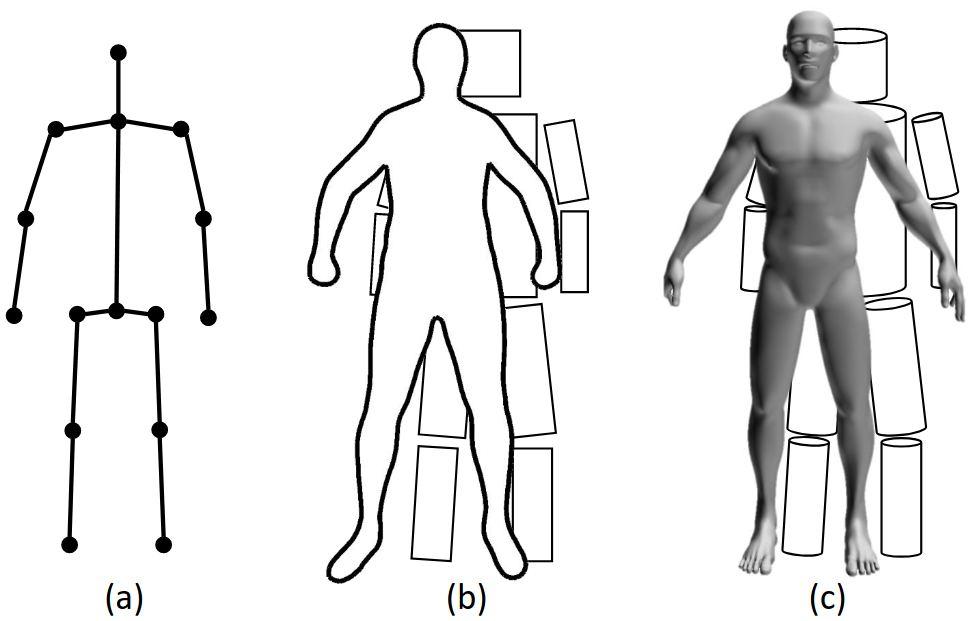
\includegraphics[width=0.6\linewidth]{figures/HPE/PoseRepresentation.png}
    \caption[Different representations of the human pose]{Different representations of the human pose. (a) Kinematic representation. (b) Contour representation. (c) 3D volume representation. \cite{HPESurveyOriginal}}
    \label{fig:pose_representation}
\end{figure}

\paragraph{Data sources}

The data that is acquired influences the way the human pose can be estimated. The most common data source is RGB images or videos. RGB videos are any videos that are captured with normal cameras that record the colour of the scene. The provided data can be either from a video or a stream of data or a still image. There is a large number of datasets that can be used to train and test poses estimation algorithms from RGB data. Some of the most common datasets are the MPII Human Pose Dataset\cite{MPII}, the COCO dataset\cite{Coco}, and HumanEva-I dataset\cite{HumanEva}.

Additionally, some datasets are captured with depth cameras. Depth cameras are cameras that can record, in addition to the colour channels, the depth of the scene. Different methods to acquire depth data have been developed. The most commonly used depth cameras emit an infrared light pattern to measure the depth of a scene. This depth information can be used to improve the accuracy of the pose estimation. Some of the most common datasets that are captured with depth cameras are the MRI dataset\cite{mRI}, and the Human3.6M dataset\cite{h36m_pami}.

Finally, there are also methods of HPE that use point clouds. Point clouds are a collection of points in space, which can be used to represent the shape of an object. Each point in the point cloud represents a point in the environment. The point cloud is created using the depth information of a scene and the intrinsics of a camera, i.e. the field of view and the focal point of the camera. A point cloud is a reconstruction of the real-world scene. Point clouds are often used in combination with RGB data. Some of the most common datasets that are captured with depth cameras are the SMMC-10 dataset\cite{SMMC10}, and the EVAL dataset\cite{EVAL}. However, any RGB and depth dataset can be used to train and test point cloud-based pose estimation algorithms if the camera intrinsics and extrinsic, such as the horizontal and vertical field of view, the focal point, and the depth units are known. With the knowledge of these parameters, the depth information can be converted to a point cloud and if the RGB data is in line with the depth data, the individual points can be coloured accordingly.

\section{Convolutional Neural Networks}

Convolutional neural networks(CNN) are a type of feed-forward neural network that are commonly used for computer vision tasks. As the name suggests, CNN apply convolutional operations in some of the layers of the network architechture. A convulutional operation is an integral over two functions to determine the amount of overlap of these functions, resulting in a third function. In CNN, the first function is usually an image or rather a matrix representation of an image and the second function is a matrix, that is changed throughout the course of network training. This operation then results in a new matrix. This is used to extract local features from an image.

In most cases, the features that are produced by multiple convolutional layers are forwarded into fully connected layers. These layers learn the features based on the input data. In case of image classification tasks, the fully connected layers are usually followed by a softmax layer to calculate the probability of each class. The class with the highest probability is then used as the prediction of the network for the given input.

Since convolutional neural networks require a lot of data to be trained properly, transfer learning is applied in some cases. Transfer learning is a technique that uses a pre-trained model to extract features from the input data. The pre-trained model is usually trained on a large dataset, such as ImageNet\cite{ImageNet}. The pre-trained model is then used to extract features from the input data. These features are then used to train a new model. This allows the new model to be trained with less data and therefore less time. Additionally, the pre-trained model is usually trained on a large dataset and therefore the features that are extracted are more general and can be used for different tasks. 

\section{Evaluation metrics}

To rightfully evaluate the performance and accuracy of a model, different metrics are used. In this section, some metrics that can be used to evaluate the performance of a model are discussed.

\subsection{Confusion Matrix}

A confusion matrix is a graph which represents the false positives and the true negatives in a single graph. The confusion matrix can be seen in table \ref{tab:confusion_matrix}. The confusion matrix is useful to visualise the performance of a model.

\begin{table}[ht]
    \caption[The Confusion Matrix]{The confusion matrix as a metric for binary classification. The results of the prediction (PRED), left, and the actual ground truth (GT), top.}
    \label{tab:confusion_matrix}
    \centering
    \begin{tabular}{l|ll}
    PRED \textbackslash GT & TRUE & FALSE \\ \hline
    TRUE                   & TP   & FP    \\
    FALSE                  & FN   & TN   
    \end{tabular}
\end{table}

\subsection{Percentage of positive Guesses}

The percentage of positive guesses is an indicator of the performance of a model. For example, if the dataset is unbalanced, the accuracy might be sufficiently good when only guessing for the majority class. In those cases, the percentage of positive guesses would either be $0\%$ or $100\%$. Therefore, the percentage of positive guesses is used to determine if the model is biased toward a specific class. The equation for the percentage of positive guesses can be seen in equation \ref{eq:percentage_of_positive_guesses}. In this thesis, the percentage of positive guesses is sometimes referred to as $\dfrac{p}{p + n}$ as it is the ratio of the number of positive guesses $p$ to the total number of guesses $p + n$.

\begin{equation}
    \label{eq:percentage_of_positive_guesses}
    \text{Percentage of positive guesses} = \frac{\text{Number of positive guesses}}{\text{Number of guesses}} = \frac{tp + fp}{tp + fp + tn + fn}
\end{equation}

\subsection{Receiver Operating Characteristic Curve}

The receiver operating characteristic curve (ROC curve) is a metric that shows the performance of a model performing binary classification tasks. It plots the true positive rate \(\frac{TP}{TP+FN}\) against the false positive rate \(\frac{FP}{FP+TN}\). This allows for the evaluation of a classifier without the influence of class distribution. An interpretation of the ROC Curve can be seen in figure \ref{fig:roc-curve}


\begin{figure}[ht]
    \centering
    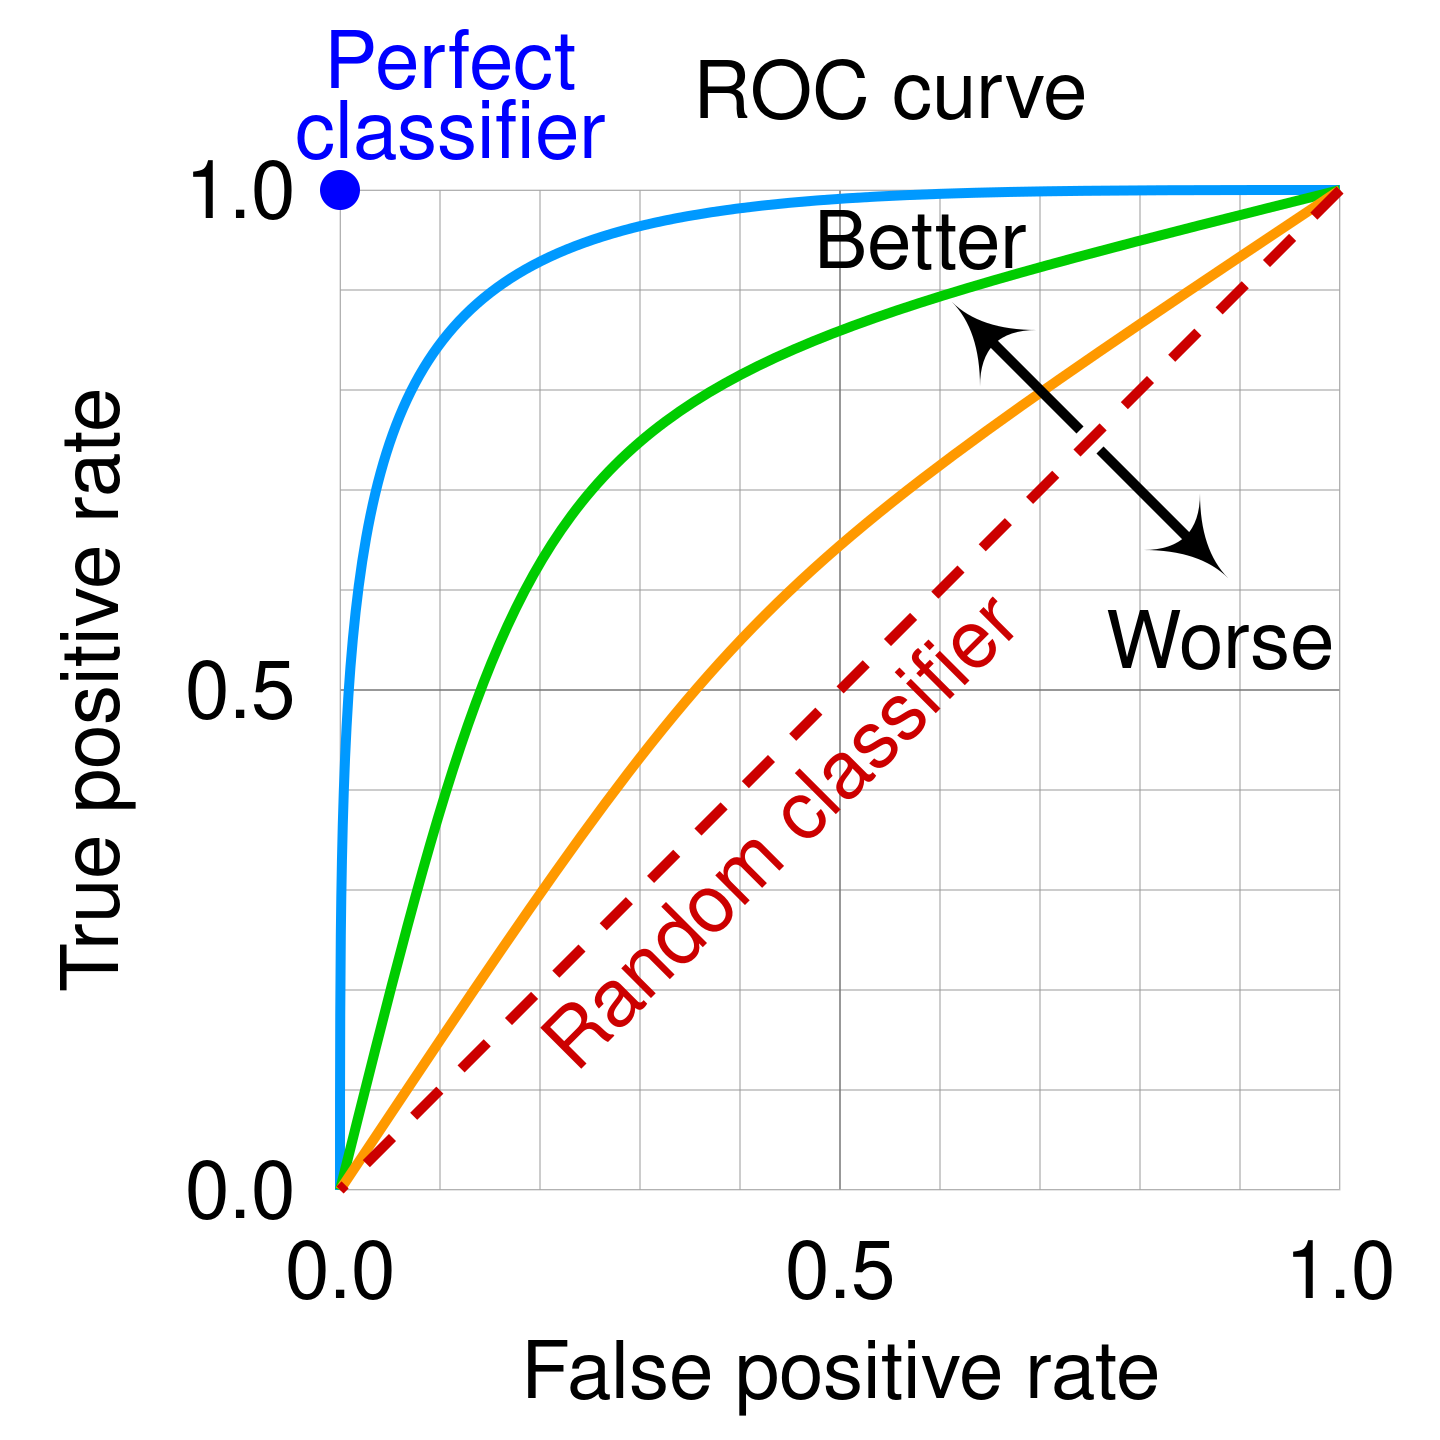
\includegraphics[width=0.5\textwidth]{figures/Roc_curve.png}
    \caption[An interpretation of the ROC Curve]{An interpretation of the ROC curve. The plotted lines are examples of exceedingly good classifiers, with orange being the worst and blue being the best.\cite{ROC-Drawing}}
    \label{fig:roc-curve}
\end{figure}
  

\subsection{Accuracy, Precision, Recall and F1-Score}

The accuracy of a prediction is the ratio of the number of correct predictions to the total number of predictions. The accuracy is calculated using equation \ref{eq:accuracy}. The accuracy is a good indicator of the performance of a model if the dataset is balanced. However, if the dataset is unbalanced, the accuracy might be sufficiently good when only guessing for the majority class. 

\begin{equation}
    \label{eq:accuracy}
    \text{Accuracy} = \frac{\text{Number of correct predictions}}{\text{Number of predictions}} = \frac{tp + tn}{tp + fp + tn + fn}
\end{equation}

The precision of a prediction is the ratio of the number of correct positive predictions to the total number of positive predictions. The precision is calculated using equation \ref{eq:precision}.

\begin{equation}
    \label{eq:precision}
    \text{Precision} = \frac{\text{Number of correct positive predictions}}{\text{Number of positive predictions}} = \frac{tp}{tp + fp}
\end{equation}

The recall of a prediction is the ratio of the number of correct positive predictions to the total number of positive samples. The recall is calculated using equation \ref{eq:recall}.

\begin{equation}
    \label{eq:recall}
    \text{Recall} = \frac{\text{Number of correct positive predictions}}{\text{Number of positive samples}} = \frac{tp}{tp + fn}
\end{equation}

Finally, the F1-Score is the harmonic mean of the precision and the recall. The F1-Score is calculated using equation \ref{eq:f1_score}. The F1-Score is a good indicator of the performance of a model if the dataset is unbalanced since it takes both the precision and the recall into account.

\begin{equation}
    \label{eq:f1_score}
    \text{F1-Score} = 2 \cdot \frac{\text{Precision} \cdot \text{Recall}}{\text{Precision} + \text{Recall}} = \frac{2 \cdot tp}{2 \cdot tp + fp + fn}
\end{equation}

\subsection{Cohen's kappa coefficient}

Cohen's kappa coefficient is an inter-rater reliability measure\cite{kappa}. This means that two different raters are compared. In the case of a binary classification, the formula for Cohen's Kappa can be seen in equation \ref{eq:kappa}. In the case of prediction, the two raters are the ground truth and the prediction.

\begin{equation}
    \label{eq:kappa}
    \kappa = \frac{2(tp \cdot tn - fn \cdot fp)}{(tp + fp)(fp+tn) + (tp + fn)(fn + tn)}
\end{equation}

If Cohens Kappa is less than 0, there is no agreement between the two raters. If the kappa score is less than 0.5 there is a slight agreement. A score of more than 0.8 is considered almost perfect. However, the "exact" values vary from application to application.